\begin{figure}[!htbp]
\centering
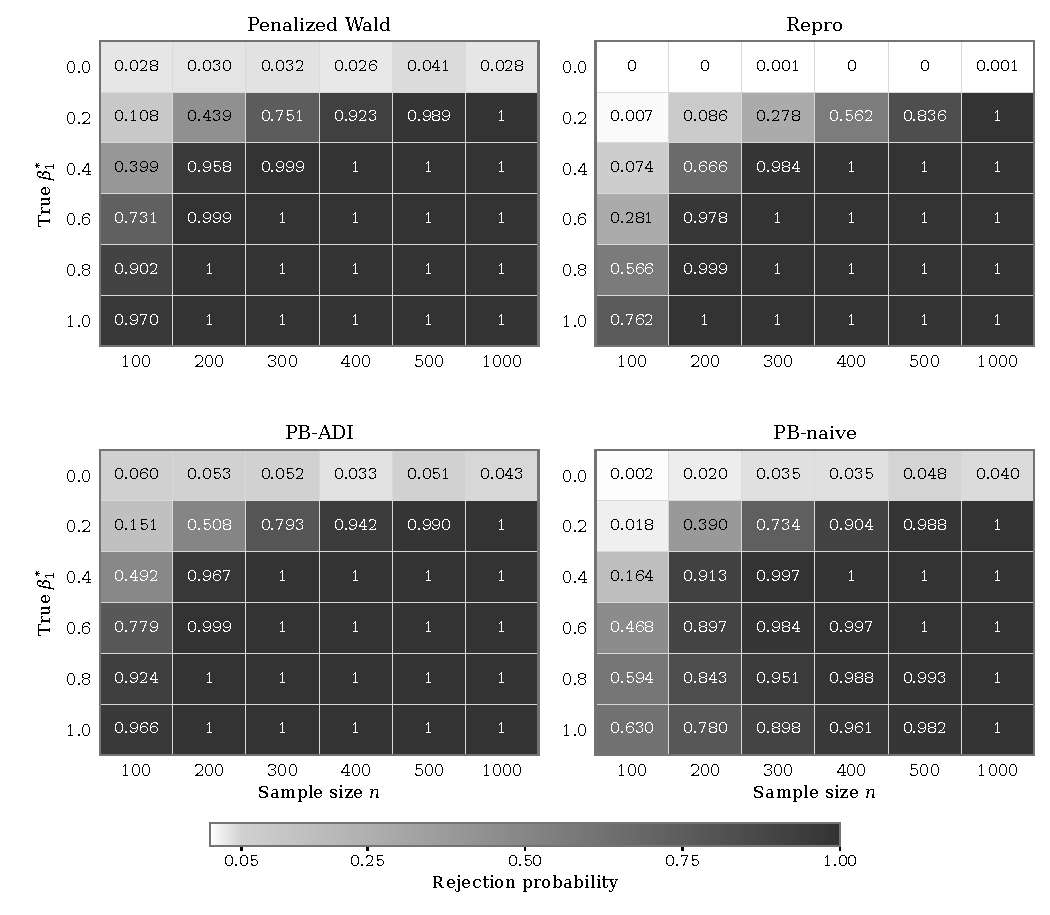
\includegraphics[width=0.95\linewidth]{results/figures/fig_exp2_comparison.pdf}
\caption{Experiment 2. Rejection probability of $H_0:\beta_1=0$ at the $0.05$ level, over $1000$ replications per cell. Rows are the true slope and columns the sample size; the bottom row of each panel is empirical size and the rest is power. The grey scale runs from $0$ to $1$ and breaks at $0.05$, so a cell at or below the nominal level is light and one above it dark. The exact finite-$R$ size bound is $0.04975$. \textsc{repro} is the procedure of Awan and Wang (2025, Fig.~5); \textsc{pb-adi} is the parametric bootstrap with the indirect estimator and approximate pivot, and \textsc{pb-naive} the plug-in bootstrap, both as reported by Wang, Chang and Awan (2026, Fig.~5).}
\label{fig:exp2-comparison}
\end{figure}
